 \documentclass[10pt,a4paper,headinclude=true,twoside]{report}
\usepackage[latin1]{inputenc}
\usepackage[a4paper]{geometry}
\usepackage{a4wide}
\usepackage{amsmath}
\usepackage{amsfonts}
\usepackage{amssymb}
\usepackage{graphicx}
\usepackage{hyperref}
\usepackage{pdflscape} % dlia landscape orientation 
\hypersetup{colorlinks,citecolor=black,filecolor=black,linkcolor=black,urlcolor=black}
\usepackage{float}
\usepackage{setspace}
\usepackage{titlesec}
\titleformat{\chapter}
  {\Large\bfseries} % format
  {}                % label
  {0pt}             % sep
  {\huge}           % before-code

\usepackage{fancyhdr}
\pagestyle{fancy}

\fancyhead[LE,RO]{\slshape  \rightmark} %should be used with "twoside" in documentcalss. Delat headeri kak v knigah: vneshnije storoni sovpadajut drug s drugom. 
\fancyhead[LO,RE]{\slshape  \leftmark}
\fancyfoot[C]{\thepage}
\lhead{}
\rhead{SE31520 Assignment: Car Insurance System}

\renewcommand{\familydefault}{\sfdefault}
\setcounter{secnumdepth}{0} % sections are level 1
\renewcommand{\thesection}{}
\makeatother
\begin{document}
\title{SE31520 Assignment: Car Insurance System}
\author{Edgar Ivanov\\ edi@aber.ac.uk \\ Department of Computer Science, Aberystwyth University}
\date{\today}
\maketitle

\newpage
\thispagestyle{empty}
\mbox{}

\tableofcontents

\section{Introduction}
There was a task to implement prototype system which would allow a user request a price quote for the car insurance. As part of this system we required to write two applications. One is underwriter which would represent insurance company and a broker which would collect quotes from the different insurance companies. However for this assignment task was simplified and broker needed to communicate just with one insurance underwriter, such approach affected some of my design decisions which I will discuss later on. For example, unique number which allows user to retrieve previous quotations is stored on the underwriter side, however in real world application it would be generated for the user and stored on the broker side and then linked to all underwriters. 

Broker and underwriter applications were developed using different technologies. For the broker I have used PHP and the underwriter had to be developed using ROR. It is a grate example of the interoperability, when applications can communicate with each other despite the fact that they are written in different programming languages and running on the different platforms. In this document I will describe design of the broker and underwriter systems, testing strategy and include self evaluation section.  

\section{Architecture of the underwriter}


%Write a section on the architecture of the underwriter application and
%rationale for decisions made. As part of this, produce a UML
%diagram(s) that shows the architecture of your application. The design
%diagram I used for the CSA application discussed in class might be a
%useful starting point. I drew mine using Powerpoint, but feel free to use
%another tool or even to draw neatly by hand!

Underwriter application was developed using Ruby on Rails and designed as a RESTful web service. It uses JSON for the representation of the content and data exchange. HTTP is used for the communication and supports all usual HTTP methods like GET, PUT, PATCH, POST, DELETE for the resource creation, deletion and so on. At the beginning I tried to implement XML support for the representation exchange but faced some issues which I couldn't overcome. After a further reading about data formats like XML, JSON, YAML I choose to use JSON since it seemed to be lightweight, human-readable and it was easy to implement support for it on the broker side.

Figure ~\ref{fig:DatabaseDesign} shows database design used to store data about the customers. Users table holds customer information like name, surname, DOB etc. Vehicles table holds information about the car: registration number, mileage, car value, it is linked to the main users table by the user\_id field and has one-to-one relationship. Since there may be a few incidents that resulted in the claim I decided to store them in the separate "driver\_history" table, this table is linked back to the customer with the user\_id field and holds information about incident date, value claimed etc., it has one-to-many relationship with the users table. Addresses table contains information about the users address and holds information like street name, postcode, country etc., it has one-to-one relationship since each user can have only one address.  

\begin{figure}[H]
\centering
\centerline{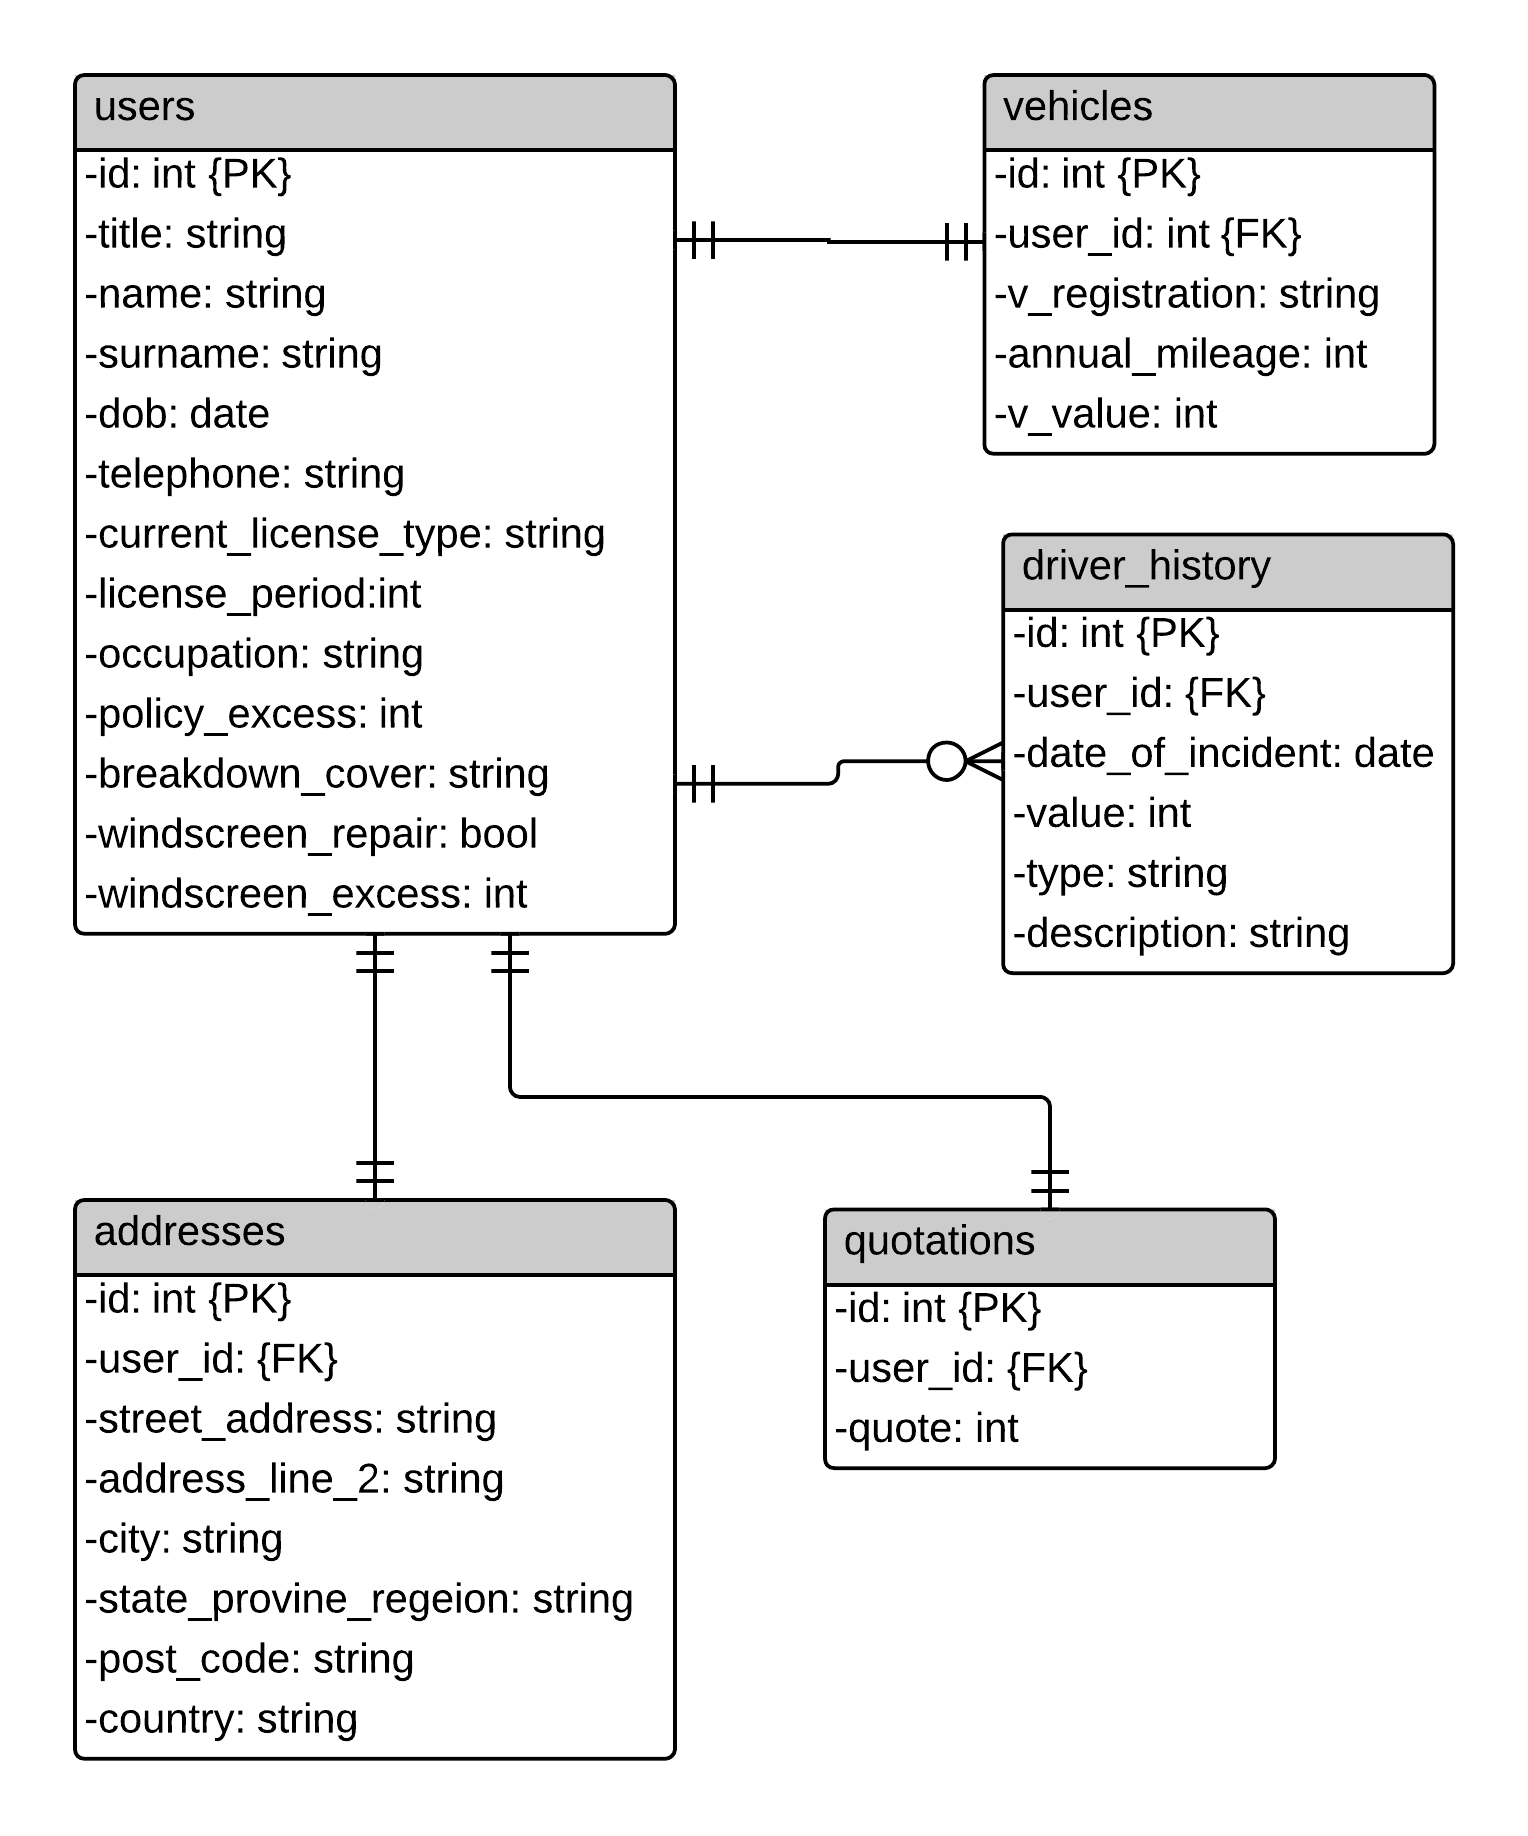
\includegraphics[scale=0.198]{./DatabaseDesign}}
\caption{Database Design}
\label{fig:DatabaseDesign}
\end{figure}

On the figure ~\ref{fig:ClassDesign} there is class digram of the underwriter application. 

\begin{figure}[H]
\centering
\centerline{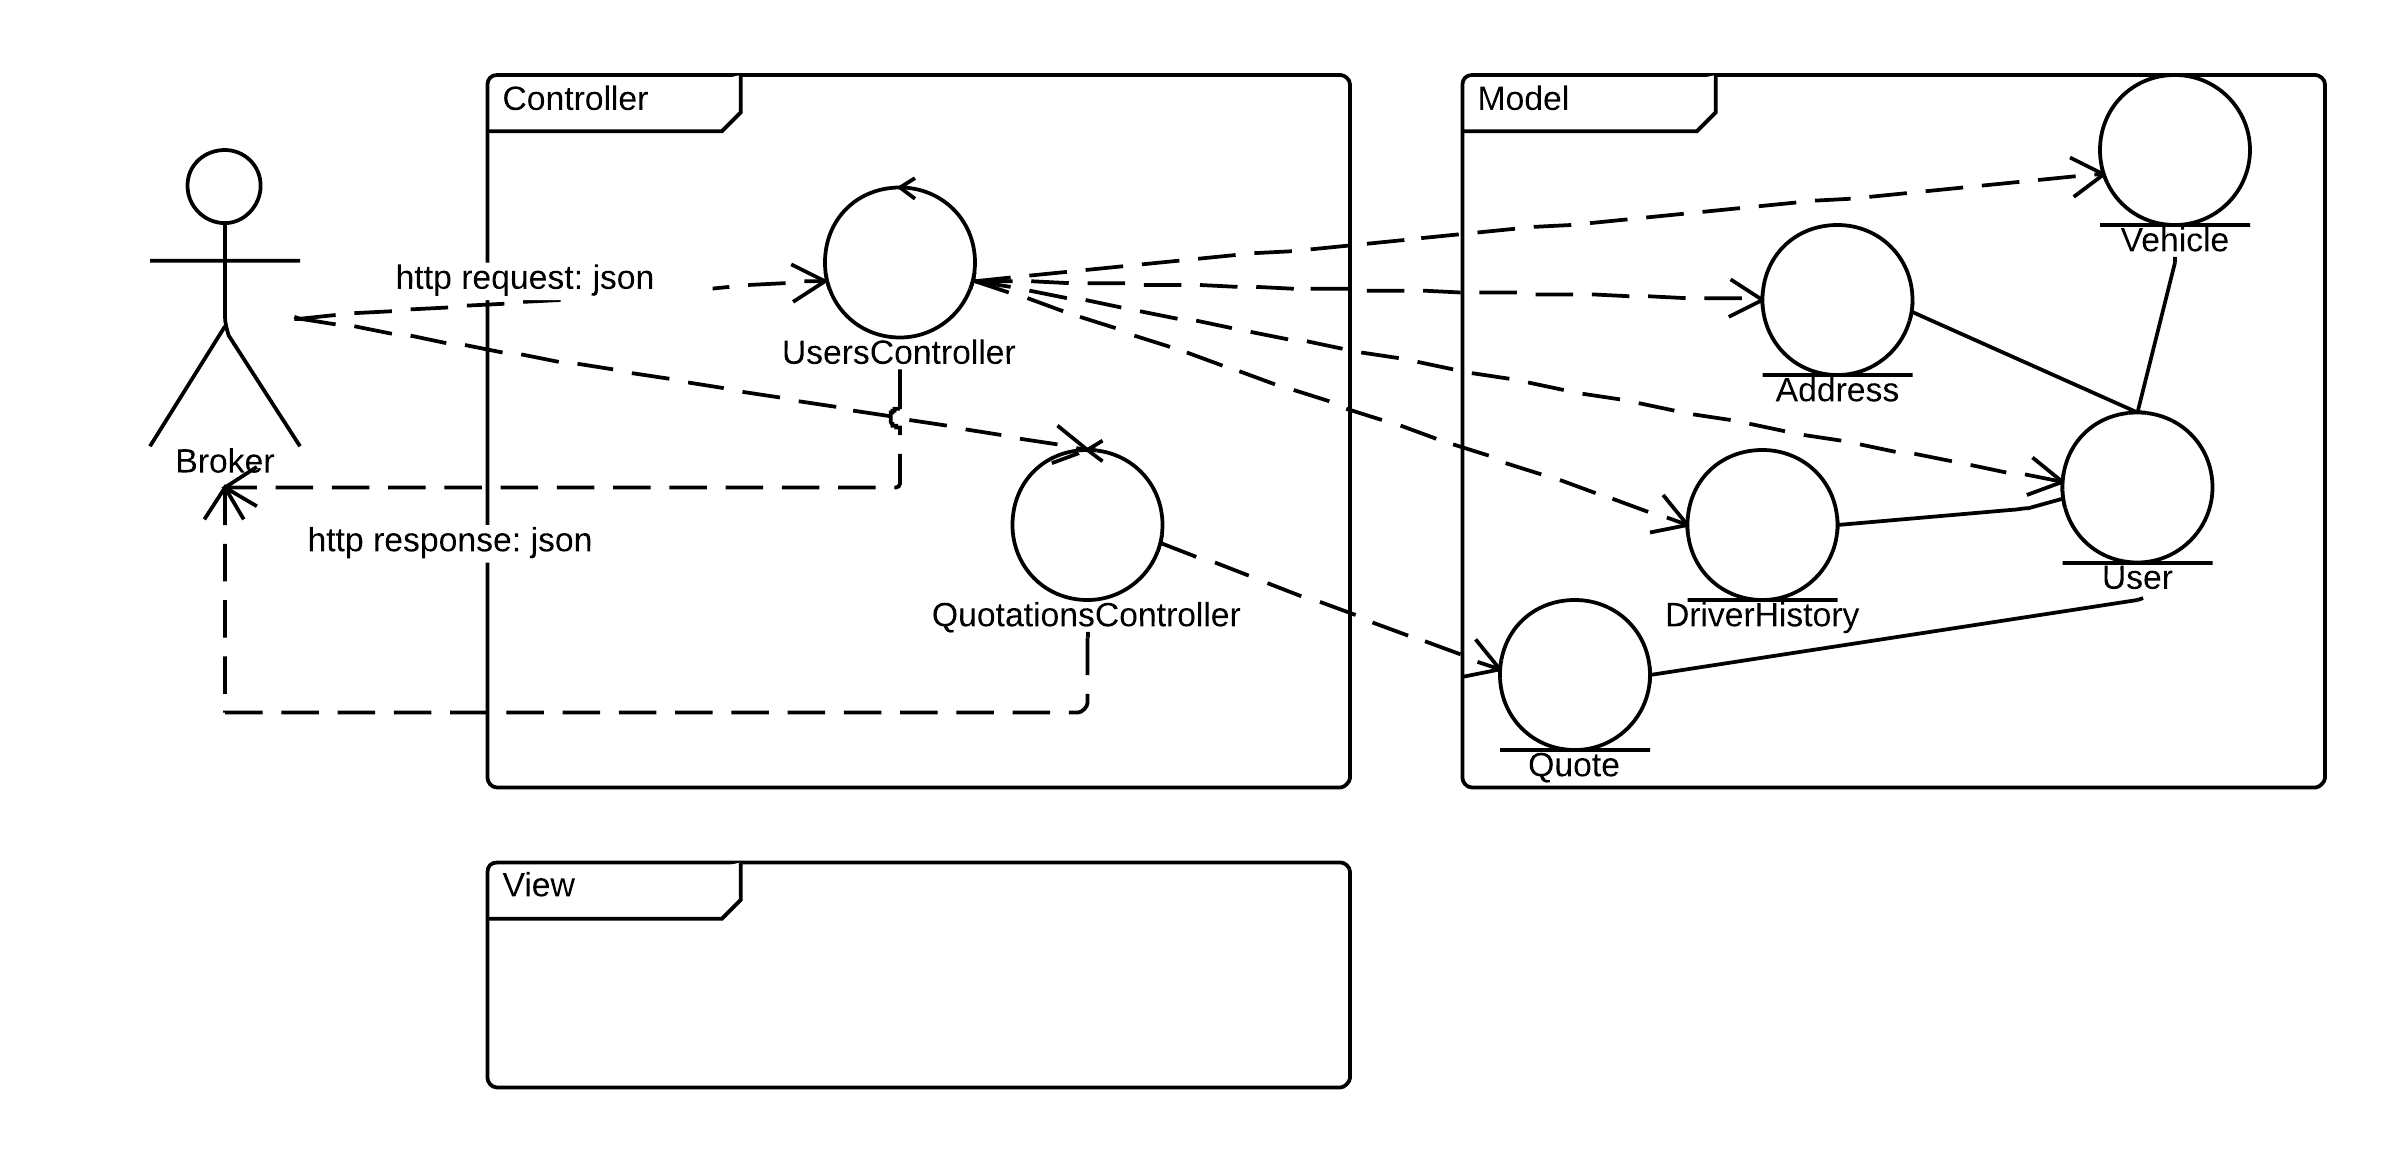
\includegraphics[scale=0.25]{./ClassDesign}}
\caption{Class Design}
\label{fig:ClassDesign}
\end{figure}


\section{Architecture of the RESTful broker}
Write a section on the architecture of the RESTful broker client,
providing rationale for decisions made.
\section{Test strategy}
Write a section on your test strategy. IMPORTANT: Provide a
screencast of your underwriter application and RESTful broker client
working (some free screen-casting tools can be found online). This
must focus on the broker to underwriter interworking and be no longer
than five minutes long.
\section{Self-evaluation}
Write a self-evaluation section. Say what mark you should be awarded
and why. Say what you found hard or easy, and what was omitted and
why. Provide an analysis of your design and the appropriateness, or
otherwise, of the technologies used.

\bibliographystyle{ieeetr}
\bibliography{bibl}

\end{document}